\documentclass{beamer}

\usepackage{tikz}
\usepackage{tkz-berge}
\usetikzlibrary{arrows.meta, petri, topaths, positioning}
\usepackage{float}
\usepackage{subcaption}
\usepackage{scrextend}
\usepackage{stackengine}
\usepackage{amsmath}
                

\title{Implementing the Solo Calculus}
\subtitle{A REPL environment for evaluation of Solo Calculus expressions}
\author{Lassiter, Adam T.}
\institute[University of Bath]{
    Department of Computer Science\\
    University of Bath
}
\subject{Computer Science}


\begin{document}

    \frame{\titlepage}



    \begin{frame}
        \frametitle{Rationale}
        \begin{itemize}
            \item Recent decline in yearly single-core performance increase of processors has led to a need to think seriously about parallelism in even everyday applications.
            \item From a theoretical viewpoint, one may wish to exhibit useful properties for multiple processes, such as equivalence of computation.
            \item What does a parallel $\lambda$-calculus look like?
        \end{itemize}
    \end{frame}



    \begin{frame}
        \frametitle{State of the Art}
        \framesubtitle{Solo Calculus}
        \begin{itemize}
            \item A calculus of communicating mobile processes.
            \item Based on Fusion Calculus, based on $\pi$-calculus, inspired by $\lambda$-calculus\ldots
            \begin{itemize}
                \item All of these have been fairly well studied so far.
                \item There exist interpreters for $\lambda$-calculus expressions, but not for any other.
                \item The suitability of the alternatives for a teaching tool is poor due to the syntax being more complicated.
            \end{itemize}
        \end{itemize}
    \end{frame}

    \begin{frame}
        \frametitle{State of the Art}
        \framesubtitle{Solo Calculus}
        \begin{center}
            \begin{tabular}{ l l l }
                Solo $\alpha \quad :=$  & $u \, \tilde{x}$              & (input) \\
                                        & $\overline{u} \, \tilde{x}$   & (output) \\ \\
                Agent $P \quad :=$      & $0$                           & (inaction) \\
                                        & $\alpha$                      & (solo) \\
                                        & $Q \, | \, R$                 & (composition) \\
                                        & $(x) \, Q$                    & (scope) \\
                                        & $Q\{x/y\}$                    & (match) \\
                                        & $!\,P$                        & (replication)
            \end{tabular}
        \end{center}
    \end{frame}

    \begin{frame}
        \frametitle{State of the Art}
        \framesubtitle{Solo Calculus}
        \begin{center}
                $\overline{x} \, y z \, | \, !(uv)(x \, u v \, | \, \overline{u} \, v) \rightarrow$ \\~\\
                $\overline{x} \, y z \, | \, (uv)(x \, uv \, | \, \overline{u} \, v) \, | \, !(uv)(x \, uv \, | \, \overline{u} \, v) \rightarrow$ \\~\\
                $(uv)(\overline{u} \, v)\{y/u, \, z/v\} \, | \, !(uv)(x \, uv \, | \, \overline{u} \, v) \rightarrow$ \\~\\
                $\overline{y} \, z \, | \, !(uv)(x \, u v \, | \, \overline{u} \, v)$
        \end{center}
    \end{frame}
   

 
    \begin{frame}
        \frametitle{State of the Art}
        \framesubtitle{Solo Diagrams}
        \begin{itemize}
            \item A canonical representation of calculus expressions.
            \item There exists an obvious analog between these algebraic `diagrams' and traditional graphical diagrams.
            \item Research led to easier calculation of replicated terms in calculi expressions.
        \end{itemize}
    \end{frame}

    \begin{frame}
        \frametitle{State of the Art}
        \framesubtitle{Solo Diagrams}
            \begin{tabular}{ l l l }
                Diagram & $\mathcal{D} \quad$ & $:= \quad triple \,\, (\mathcal{G}, \mathcal{M}, \mathcal{L})$ \\~\\

                Graph   & $\mathcal{G} \quad$ & $:= \quad multiset \,\, \{\mathcal{E}\}$ \\
                Boxes   & $\mathcal{M} \quad$ & $:= \quad multiset \,\, \{\mathcal{B}\}$ \\
                Label   & $\mathcal{L} \quad$ & $:= \quad map \,\, \mathcal{N} \in \mathcal{G} \mapsto \mathcal{N}$ \\~\\

                Edge    & $\mathcal{E} \quad$ & $:= \quad tuple \,\, (\mathcal{N}, \mathcal{N}_1~\ldots \mathcal{N}_n)_{s \in \{i, o\}}$ \\
                Box     & $\mathcal{B} \quad$ & $:= \quad pair \,\, (\mathcal{G}, set \,\, \{\mathcal{N}\})$
            \end{tabular}
    \end{frame}
    
    \begin{frame}
        \frametitle{State of the Art}
        \framesubtitle{Solo Diagrams}
        \begin{figure}[H]
            \centering
            \begin{subfigure}{0.27\linewidth}
                \centering
                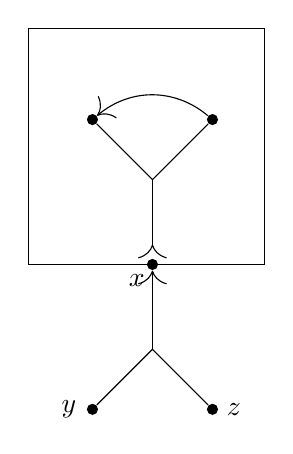
\begin{tikzpicture}[transform shape, every node/.style={circle, fill=black!100, inner sep=0.05cm}]
                    \coordinate[anchor=center](nw);
                    \coordinate[below=3cm of nw](sw);
                    \coordinate[right=3cm of nw](ne);
                    \coordinate[below right=3cm and 3cm of nw](se);
                    \draw[-] (nw) -- (ne) -- (se) -- (sw) -- (nw);
                    \node[right=1.5cm of sw, label=below left:{$x$}](x){};
                    \coordinate[below=1cm of x](xba){};
                    \coordinate[above=1cm of x](xaa){};
                    \node[above left=1cm of xaa](v){};
                    \node[above right=1cm of xaa](w){};
                    \node[below left=1cm of xba, label=left:{$y$}](y){};
                    \node[below right=1cm of xba, label=right:{$z$}](z){};
                    \draw[-{<[scale=2]}] (xaa) -- (x);
                    \draw[-{>[scale=2]}] (xba) -- (x);
                    \draw[-{>[scale=2]}] (w) to [out=140, in=40] (v);
                    \draw[-] (w) -- (xaa) -- (v);
                    \draw[-] (y) -- (xba) -- (z);
                \end{tikzpicture}
            \end{subfigure}
            $\rightarrow$
            \begin{subfigure}{0.27\linewidth}
                \centering
                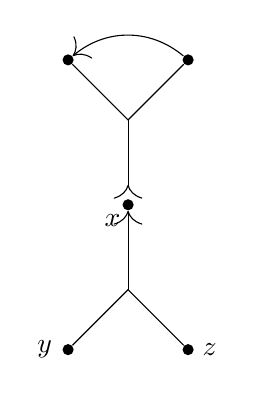
\begin{tikzpicture}[transform shape, every node/.style={circle, fill=black!100, inner sep=0.05cm}]
                    \coordinate[anchor=center](nw);
                    \coordinate[below=3cm of nw](sw);
                    \coordinate[right=3cm of nw](ne);
                    \coordinate[below right=3cm and 3cm of nw](se);
                    \node[right=1.5cm of sw, label=below left:{$x$}](x){};
                    \coordinate[below=1cm of x](xba){};
                    \coordinate[above=1cm of x](xaa){};
                    \node[above left=1cm of xaa](v){};
                    \node[above right=1cm of xaa](w){};
                    \node[below left=1cm of xba, label=left:{$y$}](y){};
                    \node[below right=1cm of xba, label=right:{$z$}](z){};
                    \draw[-{<[scale=2]}] (xaa) -- (x);
                    \draw[-{>[scale=2]}] (xba) -- (x);
                    \draw[-{>[scale=2]}] (w) to [out=140, in=40] (v);
                    \draw[-] (w) -- (xaa) -- (v);
                    \draw[-] (y) -- (xba) -- (z);
                \end{tikzpicture}
            \end{subfigure} 
            $\rightarrow$
            \begin{subfigure}{0.27\linewidth}
                \centering
                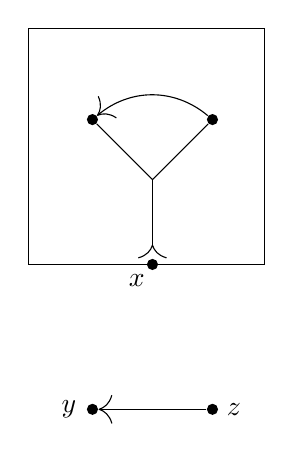
\begin{tikzpicture}[transform shape, every node/.style={circle, fill=black!100, inner sep=0.05cm}]
                    \coordinate[anchor=center](nw);
                    \coordinate[below=3cm of nw](sw);
                    \coordinate[right=3cm of nw](ne);
                    \coordinate[below right=3cm and 3cm of nw](se);
                    \draw[-] (nw) -- (ne) -- (se) -- (sw) -- (nw);
                    \node[right=1.5cm of sw, label=below left:{$x$}](x){};
                    \coordinate[below=1cm of x](xba){};
                    \coordinate[above=1cm of x](xaa){};
                    \node[above left=1cm of xaa](v){};
                    \node[above right=1cm of xaa](w){};
                    \node[below left=1cm of xba, label=left:{$y$}](y){};
                    \node[below right=1cm of xba, label=right:{$z$}](z){};
                    \draw[-{<[scale=2]}] (xaa) -- (x);
                    \draw[-{>[scale=2]}] (w) to [out=140, in=40] (v);
                    \draw[-] (w) -- (xaa) -- (v);
                    \draw[-{>[scale=2]}] (z) -- (y);
                \end{tikzpicture}
            \end{subfigure}
            \caption*{\tiny$\overline{x}\, y z \, | \, !(uv)(x \, u v \, | \, \overline{u} \, v) \longrightarrow
                            \overline{x}\, y z \, | \, (uv)(x \, u v \, | \, \overline{u} \, v) \, | \, !(uv)(x \, u v \, | \, \overline{u} \, v) \longrightarrow
                            \overline{y} \, z \, | \, !(uv)(x \, u v \, | \, \overline{u} \, v)$}
        \end{figure}
    \end{frame}



    \begin{frame}
        \frametitle{Methods and Results}
        \begin{itemize}
            \item Datatypes implementing Solo Calculus expressions and operations
            \item Simple Read-Eval-Print-Loop interface for inputting expressions and computing reductions
            \item Datatypes for Solo Diagrams and (some) operations
            \item Proof-of-Concept for Diagram visualisation
            \item Demonstration at the end~\ldots
        \end{itemize}
    \end{frame}



    \begin{frame}
        \frametitle{Plans Moving Forward}
        \begin{itemize}
            \item Completion of Solo Diagrams operations (full reduction semantics)
            \item Possible conversion between Diagrams and Calculus expressions
            \item Realtime visualisation of Diagrams using Javascript's D3 library
        \end{itemize}
    \end{frame}



    \begin{frame}
        \frametitle{Demonstration Time}
        \begin{center}
            Any questions~\ldots?
        \end{center}
    \end{frame}

\end{document}
